\chapter{Introduction}

\section{Overview}

The atmosphere is a complicated system, and numerous elements, including air particles, solid and liquid molecules, influence the extinction effect. Air pollution is a worldwide crisis with limited solutions that is caused because of the presence of compounds in the atmosphere that are detrimental to the wellness of habitants, or pose a hazard to the ecosystem or objects. Starting from long term damage to the built environment to exposure of buildings to pollutants causing degradation, changes in soiling patterns due to rain impingement and corrosion metal and glass was discovered (Brimblecombe, n.d., #).  

Air pollutants have been reported differing in their chemical composition, reaction properties, emission, persistence in the environment, ability to be transported in long or short distances. However, variants of polluting compounds with similar properties have been divided into four categories (Castanas & Kampa, 2007, #). The main anthropogenic sources are as follows : 

\begin{enumerate}
\item Gaseous contaminants. 
Compounds like SO2, NOx, CO, ozone, Volatile Organic Compounds are the prime forms of air pollutants, which form due to combustion of fossil fuels, leakage of chemicals into the atmosphere in the making process of advanced technologies. 

\item Persistent organic pollutants.
Atmospheric toxins like dioxins are emitted in the atmosphere during incomplete combustion and whenever materials containing chlorine (e.g. plastics) are burned. Heavy metals like lead and mercury are natural components of the earth’s crust, thus they cannot be degraded or destroyed and can only be transported by air - infiltrating water and human food supply. Furthermore, toxins affect the atmosphere from a range of sources, such as combustion, waste water discharges and production plants.

\item Particulate Matter.
This is the vital reason for cardiovascular, respiratory diseases leading to damaging of the nervous system since it is very tiny in size. The major sources of particulate pollution are factories, power plants, refuse incinerators, motor vehicles, construction activity, fires, and natural windblown dust. 

\end{enumerate}

The rising fossil fuel combustion over the last century is to be accountable for the gradual change in climate patterns, which lead to air pollution. Intense toxic substance discharge to the environment by mostly the developing countries of Annex B of the Kyoto Protocol are responsible for being the prime sources of pollution - since their focus is to expand industrial areas on a larger scale, overuse of power generation and introducing advanced technologies in their countries which can elevate them from 3rd world countries. The industrial revolution has occurred across every region of the globe as a response to the expansion in mechanization and automation has enhanced the standards of living for some citizens while also adding to the country's economic progress.  Apart from anthropogenic acts, several physical activities (volcanoes, fires, etc.) emit various pollutants into the biosphere, which also contributes equally to higher emission of GHG gases. 

\section{Objectives}

The notion of our project is not against the development revolution of 3rd world countries - our goal is to spread awareness globally to make toxic discharge in a favourable amount. With Dhaka being entitled as one of the top most polluted cities among 106 countries according to IQAir from 2019 and onwards, the main objective of our research is to help fulfill the 13th SDG goal - Climate Action,  with the help of IoT. For the introduction of automation, the idea of Industrial IoT (IoT) acquired significant attention. While this aspires to boost productivity, efficiency and real-time visibility, IoT has become the most desirable field of research.Iot is a system of interrelated devices connected to the internet to transfer and receive data from one to the other and enables device-to-device and human-to-device interactions in a reliable and robust manner. 

This project focuses is to improve air quality and to establish a mechanism to improve AQI by monitoring the air standard. Our goal is to diminish the problem efficiently within the limited resources economically.


\section{Scopes}

Our scope is to make an economically friendly device, predict PM2.5 concentration using satellite data with the help of Machine Learning and make a software as an atmospheric forecast reporting system using the device and satellite data.

This research is proposing two types of solutions to mitigate the worldwide crisis.It will consist of retrieving data from a primary source where IoT will be implemented, and a secondary source where data from AQUA satellite is extracted. The main objective of this paper is to make an inexpensive solution to the problem, which will be then compared with an industrial graded expensive device to determine the device compatibility. Additionally, we have to make sure to measure the air quality of all the regions of Bangladesh. Our aim is to make a software as an atmospheric forecast reporting system, where we intend to incorporate station wise-graphs using device and satellite data and generate a ‘AQI alert Atmospheric Map’. The diagram below shows a preliminary model of the proposed system.

\begin{figure} [H]
    \centering
    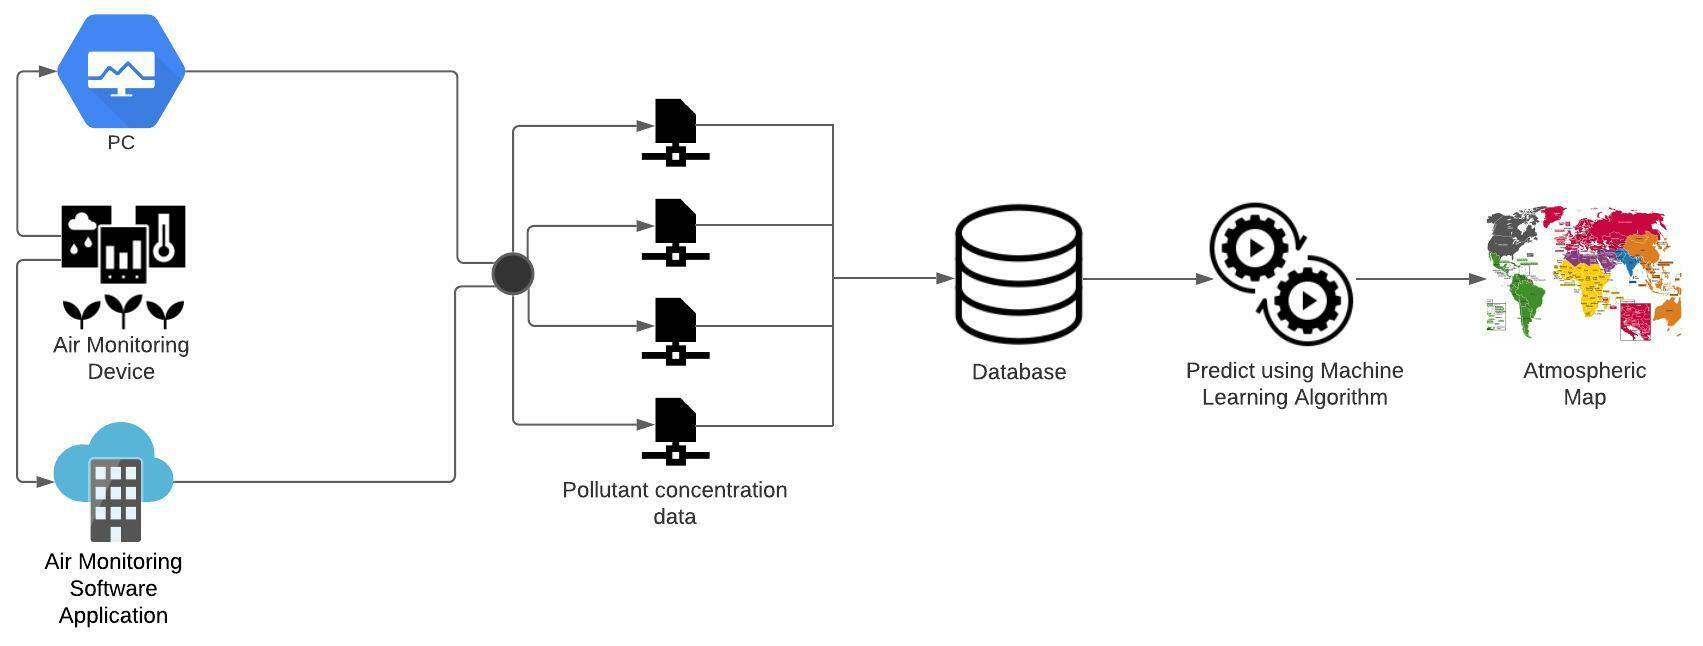
\includegraphics[width=\textwidth]{images/1_1_System Design AQM.jpeg}
    \caption{Proposed System detailed representation diagram}
    \label{fig:System Design AQM}
\end{figure}

In this paper, for the primary data, IoT has been proposed for the detection of polluting compounds in our atmosphere causing global warming and calculating the AQI with the help of data we get from the sensors that detect the toxic gas. The project intends to measure the temperature, humidity, barometric pressure, VOCs, multiple toxic gases and detect concentration of fine particles smaller than 1.0μm, 2.5μm and 10.0μm in diameter. With the set of sensors connected to the development board, Arduino Mega 2560 Wifi takes readings from the sensors and sends all the sensor data to the PC using Serial Communication. This data is then migrated to the cloud. All the concentration of polluting compound charts will be shown in a Google Sheet visualization for now. 

Afterwards our intention is to compare the primary data of the pollutants with an industrial graded device by IQAir, to determine the device precision. Coming onto the industrial graded device we have purchased, AirVisual Pro -  the vital goal of the IQAir technology is to operate the world’s largest real time air quality platform. Not only has it taken the initiative to help people explore every country’s real time air quality remotely through a world pollution map, but also has made it easier and more accessible to people to do instant indoor air quality monitoring by launching an application. Overall, the data of this device is known to have good accuracy and is used by people as a reference. 

\begin{figure} [H]
    \centering
    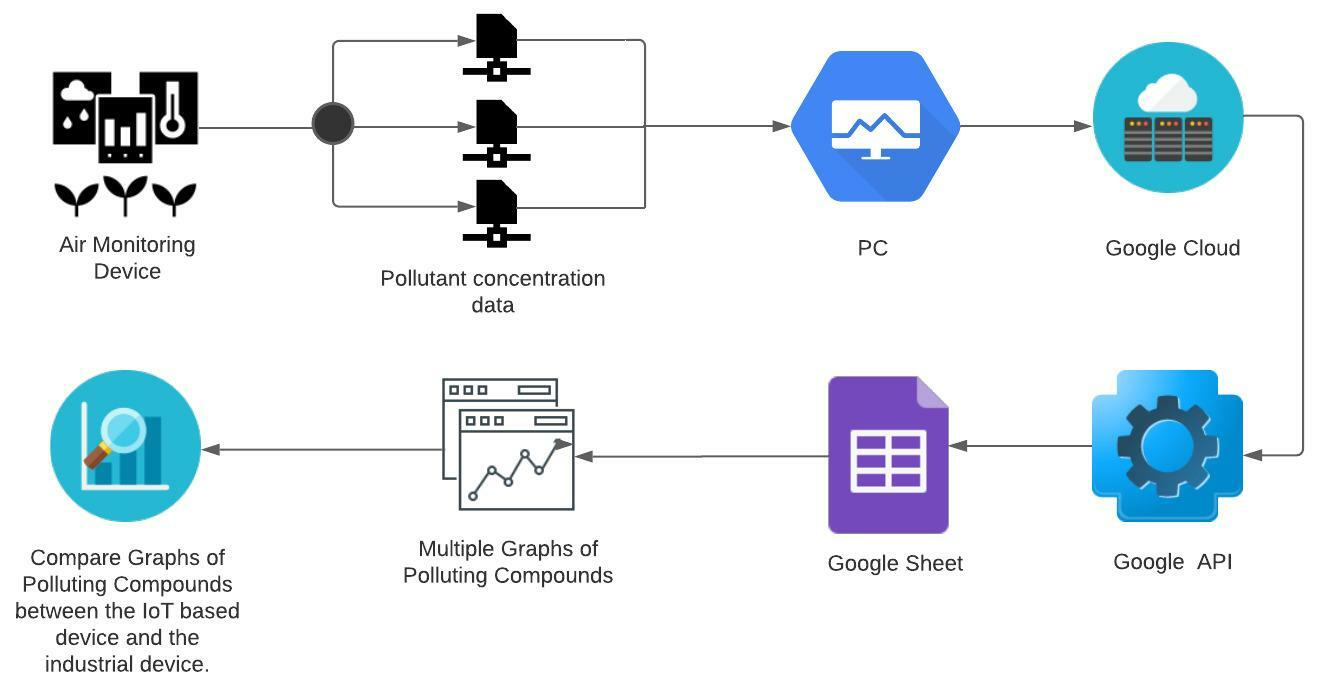
\includegraphics[width=\textwidth]{images/1_2_System Design RefinAir.jpeg}
    \caption{IoT based device detailed representation diagram}
    \label{fig:System Design RefinAir}
\end{figure}

In the process of covering all the areas of Bangladesh, the inexpensive device that we will be making will no longer be cost efficient since we have to expand the infrastructure. To solve this problem, a successful approach has been noted from multiple research where the secondary data - AOD PM2.5 product - is predicted using Machine Learning Algorithms (MLAs).

The secondary data is originally extracted from the Bangabandhu Satellite, which happens to be the only satellite in Bangladesh with two ground stations. The main ground station is in Gazipur’s Telipara and the alternate backup Earth ground station is in Rangamati’s Betbunia. The AOD (Aerosol Optical Depth) 550 nm data is collected and preprocessed by the AQUA satellite using the MODIS(Moderate Resolution Imaging  Spectroradiometer) instrument while orbiting above Bangladesh. AOD is the measure of  550 nm aerosols (e.g., urban haze, smoke particles, desert dust,  sea salt) distributed within a column of air from the Earth’s surface to the top of the atmosphere. The  used AOD 550 nm is the dust aerosol optical thickness at 550 nanometers (nm). The satellite AOD  (Aerosol Optical Depth) 550 nm data was collected using NASA Giovanni data visualization platform. 

In the process of making an atmospheric forecast reporting system, we aspire to make a software incorporated with the device. We intend to integrate station wise graphs and using MLAs our aim is to generate an ‘AQI alert Atmospheric Map’,with the help of the satellite and device data. Additionally, our project will extensively monitor the most polluting areas/routes - to give an alert when the pollution exceeds the favourable amount.

\begin{figure} [H]
    \centering
    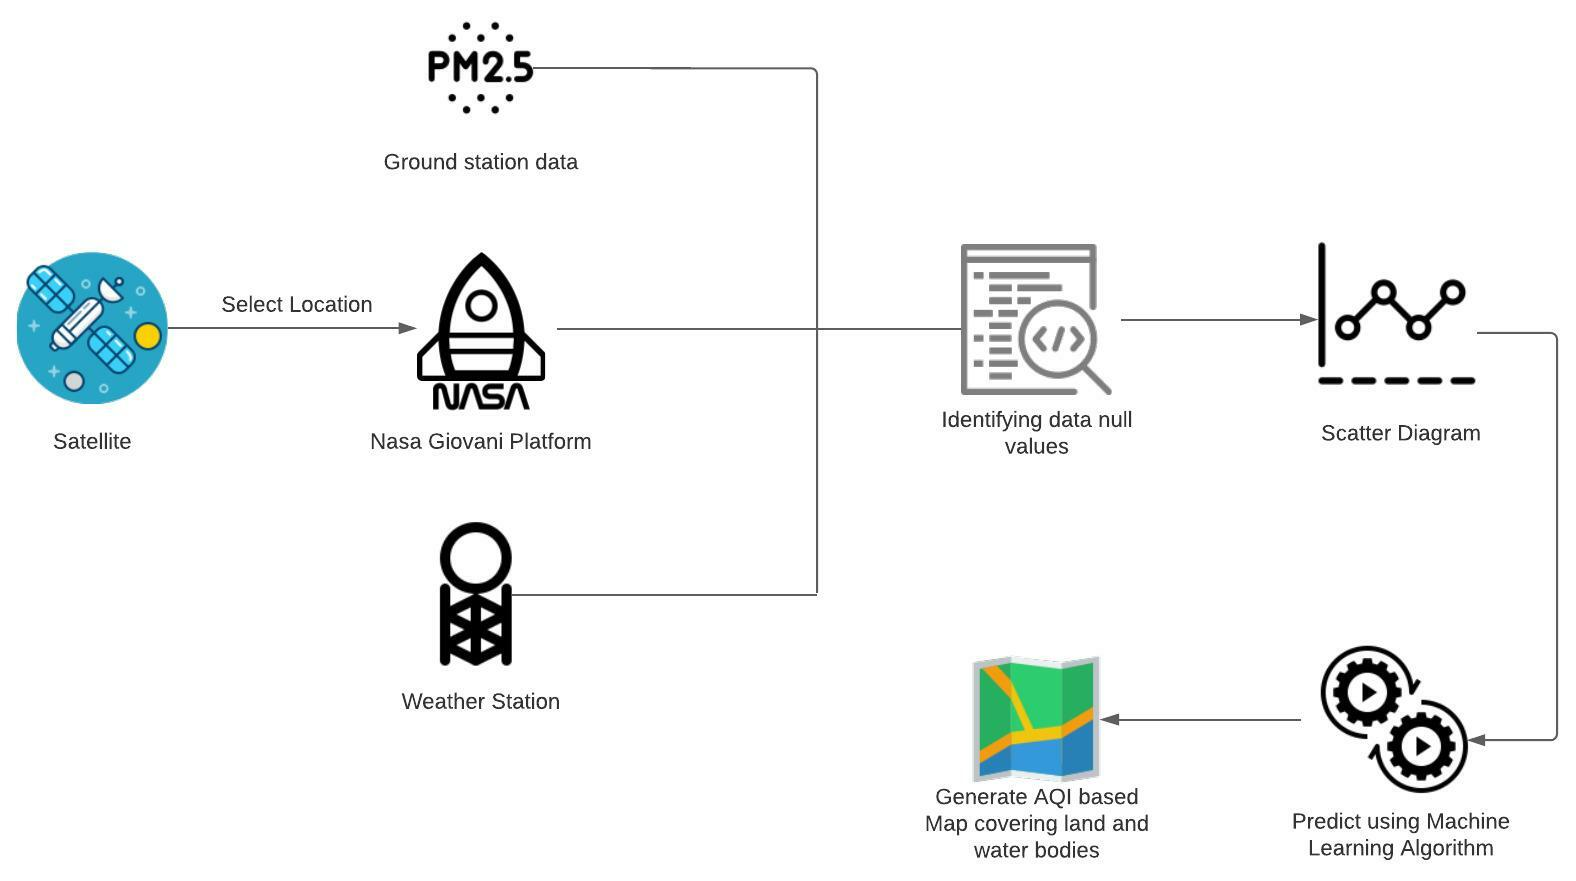
\includegraphics[width=\textwidth]{images/1_3_System Design Satellite .jpeg}
    \caption{Prediction of PM2.5 concentration using Satellite data detailed representation diagram}
    \label{fig:System Design Satellite}
\end{figure}

\section{Organization of the report}

In this section, we are going to determine the contents of the chapters in this paper. 

The ‘Chapter 1’ denotes the introductory part of the research to give a clear idea and overview of the project. It also contains the scope of the project, where our targets for this research are discussed.

In the ‘Chapter 2’ section, the literature reviews on multiple papers will be done to find out the possibilities to achieve the goals of this project and this will help us build our knowledge in this field. The literature review will be divided into two sub-sections : one for the IoT based device and another for the satellite data.

Moving on to ‘Chapter 3’, it will contain the project breakdown, timings and schedules along with roles and responsibilities. It means to achieve goals and involves decision making, keeping in mind about all the potential risks and finding ways to diminish them by doing a critical path analysis.

The hypothesis of a vital part from our research will be found in ‘Chapter 4’. It will describe the problem statement to introduce the readers to the importance of the topic being studied. A step by step proposed system is added to this chapter to gain the consensus of the readers about the project. 

The primary data source, IoT based Device which is also known as RefinAir, is discussed in ‘Chapter 5’. An introduction is given on the device and AirVisual Pro together to help the readers correlate the purpose of the project. Since the IoT based Device itself is a prototype, our aim is to make a pre-prototype for our desired system, to give a representation of the design of the finalized system. In the problem statement sub-section, we will present the expensive air quality devices available in the market as a problem and will express our desire to make an inexpensive device as a solution. Also, we will point out the fact that we will try to make our device more durable and sustainable and easier to maintain for the users. Another sub-section is made for the system description where the chosen device components are justified by comparing it with other industrially approved components. A hardware layout is shown using block and schematic diagrams - followed by the original picture of the hardware which will be assembled by us using the components. Afterwards, a performance analysis will be done to compare the data of the polluting compounds measured by both the IoT based device and AirVisual Pro. Both daytime and nighttime data will be taken to determine the data accuracy and IoT based device compatibility. Application of RefinAir will be stated and an overall comparison will be done between AirVisual Pro and RefinAir based on the difference between the functionalities and facilities given by them.

The prediction on  PM2.5 data concentration using Machine Learning will be shown in the ‘Chapter 6’, where the collection of AOD and ground station data is discussed and the procedure to convert AOD 550 nm to PM2.5 data is stated. In this section, we will determine which Machine Learning Algorithms works best for prediction analysis of PM2.5 concentrations. All the Machine Learning Algorithms used and their outcomes will be discussed here.

In the last part, ‘Chapter 7’, the challenges faced are discussed for the hypothesis, primary data and the secondary data. The environmental, ethical and social issues are declared here. Authors’ interest in developing new proposals based on the same research are affirmed in the future work and recommendation sub-section.
